\documentclass[10pt,conference]{IEEEtran}

\IEEEoverridecommandlockouts
\usepackage{cite}
\usepackage{graphicx}
\usepackage{booktabs}
\usepackage{tabularx}
\usepackage{listings}
\usepackage{xcolor}
\usepackage{url}
\usepackage[hidelinks]{hyperref}

\definecolor{codebg}{RGB}{245,245,245}
\lstdefinestyle{tool}{
  basicstyle=\ttfamily\footnotesize,
  backgroundcolor=\color{codebg},
  frame=none,
  xleftmargin=4pt,
  xrightmargin=4pt,
  breaklines=true,
  columns=fullflexible,
  keepspaces=true,
  showstringspaces=false,
}
\lstset{style=tool}

% Tool name, typeset consistently.
\newcommand{\tool}{\textit{civic-tech-crawler}}

\begin{document}

\title{civic-tech-crawler: A Lightweight CHAOSS-Aligned Repository Mining Tool with AI-Usage Detection}

\author{%
  \IEEEauthorblockN{Janne Parkkila}
  \IEEEauthorblockA{LUT University\\
  Lappeenranta, Finland\\
  Janne.Parkkila@lut.fi}
  \and
  \IEEEauthorblockN{Viktoriia Olshanskaia}
  \IEEEauthorblockA{LUT University\\
  Lappeenranta, Finland\\
  viktoriia.olshanskaia@lut.fi}
  \and
  \IEEEauthorblockN{Duc Thinh Tran}
  \IEEEauthorblockA{LEGO, IMT Atlantique, Brest, France\\
  LUT University, Lappeenranta, Finland\\
  Duc-Thinh.Tran@imt-atlantique.fr}
  \and
  \IEEEauthorblockN{Antti Knutas}
  \IEEEauthorblockA{LUT University\\
  Lappeenranta, Finland\\
  Antti.Knutas@lut.fi}
}

\maketitle

\begin{abstract}
Existing repository-mining platforms such as GrimoireLab and Augur assume an Elasticsearch or database stack that is disproportionate for studies of a few dozen repositories, and none of them treats traces of AI coding agents as a first-class signal. We present \tool{}, a Python command-line tool that collects 25+ CHAOSS and DORA indicators, per-contributor weekly effort, and an AI-usage layer that separates AI-assisted development from shipped LLM features and active use from merely declared intent. The tool falls back to the full commit history when GitHub's asynchronous statistics endpoints fail to answer, which in our most recent crawl happened for 50 of 55 repositories. It is configured by a single YAML file, distributed as a Python package and a Docker image with host-side mounts, and covered by 83 unit tests under continuous integration. \tool{} produced a Zenodo-archived corpus of 55 civic-technology projects that underpins a published empirical study of the civic-tech landscape. This paper describes the tool itself: its architecture, the design decisions behind the coverage fallback and the AI-usage layer, and tool-level validation evidence.
\end{abstract}

\begin{IEEEkeywords}
mining software repositories, CHAOSS, AI-assisted development, civic technology, open-source sustainability
\end{IEEEkeywords}

\section{Introduction}

Mining tooling for open-source research is mature for the large-ecosystem case. GrimoireLab~\cite{grimoirelab} integrates some 30 data sources through an Elasticsearch/Kibana stack and powers the CHAOSS dashboards~\cite{chaoss}; Augur~\cite{augur} runs as a long-lived PostgreSQL-backed service with a web interface; Perceval~\cite{perceval} is GrimoireLab's retrieval layer. Each assumes infrastructure that a researcher studying a defined sample of 30--100 repositories does not need and cannot easily version-control alongside the analysis scripts.

A second gap is recent. The 2025--2026 wave of agentic developer tooling (Claude Code, GitHub Copilot's coding agent, Devin, Jules, Cursor) leaves observable traces in repositories: agent instruction files, commit co-author trailers, and pull requests opened by agent accounts. Mainstream mining tools do not expose these traces as a metric family, so studies of how AI tooling is actually adopted in open source must build ad-hoc detectors.

\tool{} addresses both gaps. It was built to study open-source civic technology~\cite{civictech}, a domain of small, often volunteer-maintained projects, but nothing in its design is civic-tech specific. It has been in use since February 2026 and produced the 55-project corpus analysed in a companion empirical paper~\cite{goodit26}, which reports the findings; this paper describes the instrument.

\textbf{Contributions.}
(1)~A lightweight, CHAOSS-aligned mining CLI configured by a single YAML file and shipped with a Docker image and continuous integration.
(2)~A coverage fallback that derives weekly activity from the full commit history when GitHub's asynchronous statistics endpoints do not respond.
(3)~An AI-usage detection layer that decomposes adoption into development versus product use and active use versus declared intent, with per-signal provenance and first-appearance dates.
(4)~A Zenodo-archived 55-project corpus produced by the tool~\cite{zenodo-dataset}.

\section{Tool Architecture}

\tool{} is a Python~3.13 package of roughly 5{,}000 lines organised in three layers (Fig.~\ref{fig:arch}). A CLI orchestrator reads the YAML configuration and iterates over the repository list; eight collectors each return a typed dataclass built from the GitHub REST and GraphQL APIs; and two exporters serialise the result to CSV files (one row per repository, contributor, issue, pull request, tag, or week) and to a single hierarchical JSON document.

\begin{figure}[t]
  \centering
  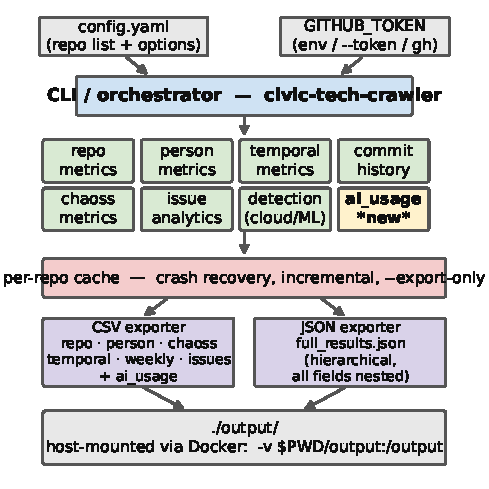
\includegraphics[width=\columnwidth]{figures/fig1_architecture.pdf}
  \caption{Architecture of \tool{}. The orchestrator runs eight collectors per repository, persists each result to a per-repository cache, and exports CSV and JSON. The highlighted \texttt{ai\_usage} collector is new in the current release.}
  \label{fig:arch}
\end{figure}

\subsection{Collectors}

Each metric family lives in its own module: \texttt{repo\_metrics}, \texttt{person\_metrics}, \texttt{temporal\_metrics}, \texttt{commit\_history}, \texttt{chaoss\_metrics}, \texttt{issue\_analytics}, \texttt{detection} (cloud and classical-ML signals), and \texttt{ai\_usage}. Collectors run in a fixed order so that later ones can reuse earlier results instead of issuing new API calls. For example, \texttt{ai\_usage} reads co-author trailers tallied by \texttt{commit\_history} during its single walk over the history, and agent-authored pull requests from \texttt{temporal\_metrics}.

\subsection{Coverage fallback for asynchronous statistics}
\label{sec:cov}

GitHub computes \texttt{/stats/commit\_activity} and \texttt{/stats/contributors} asynchronously: a request for uncached statistics returns HTTP~202 and the client is expected to retry. In practice these endpoints are unreliable. During the 2026-06 crawl, \texttt{/stats/commit\_activity} returned no data within the retry budget for 50 of the 55 repositories, including large, active projects. An analysis that relied on the endpoint would have weekly activity for five repositories, and the subset that does return is not a random sample, which invites selection bias.

\tool{} therefore runs \texttt{commit\_history} before \texttt{chaoss\_metrics}. It walks the complete history through the commits API, which does not depend on the statistics cache, and aggregates commits and changed lines into ISO-week buckets per author. When \texttt{/stats/commit\_activity} yields nothing, \texttt{chaoss\_metrics} derives burstiness, weekly activity, and newcomer rates from these buckets and logs that it did so.

\subsection{Bot detection}

Concentration metrics are distorted by automation accounts. A transparent detector matches the \texttt{[bot]} suffix of GitHub Apps and an allowlist of common automation accounts (Dependabot, Renovate, GitHub Actions, Snyk, Mergify, SonarCloud, Coveralls, and others). We chose a rule-based detector over a learned classifier~\cite{golzadeh-bots} so that results are reproducible and auditable. Bus factor, elephant factor, and the Herfindahl--Hirschman index (HHI) are emitted both with and without bots, together with per-repository bot contributor and commit counts.

\subsection{AI-usage detection}
\label{sec:ai}

The \texttt{ai\_usage} collector separates two dimensions.

\textbf{Development vs.\ product.} The \emph{dev} group records evidence that AI helped build the code: agent instruction files (\texttt{CLAUDE.md}, \texttt{AGENTS.md}, \texttt{GEMINI.md}, \texttt{.cursorrules}, \texttt{.cursor/rules}, \texttt{.windsurfrules}, \texttt{.clinerules}, \texttt{.github/copilot-instructions.md}, among others); \texttt{Co-authored-by} trailers naming an AI tool; commits and pull requests authored by agent accounts such as \texttt{copilot-swe-agent[bot]} and \texttt{devin-ai-integration[bot]}; CI workflows invoking AI actions; and AI review bots. The \emph{product} group records evidence that the project ships LLM functionality, chiefly LLM provider SDKs (OpenAI, Anthropic, Cohere, and others) in dependency manifests.

\textbf{Active use vs.\ declared intent.} A project with an agent instruction file but no AI-attributed commits or pull requests has declared intent; one with AI-attributed contributions shows active use. Counting configuration files alone would overstate practised AI development.

\textbf{Provenance.} Every signal is a row with its group, tool, evidence source (\texttt{file}, \texttt{commit\_trailer}, \texttt{commit\_author}, \texttt{pr\_author}, \texttt{pr\_body}, \texttt{workflow}, \texttt{dependency}, \texttt{topic}, \texttt{bot\_comment}), the concrete evidence, a count, and a first-appearance date where one exists. Sources are graded as strong (files, trailers, agent authorship), medium (workflows, PR bodies, dependencies), or weak (topics). The vocabulary is a default that can be overridden from the YAML configuration, so new tools can be added without code changes. The collector writes \texttt{ai\_usage.csv} (one row per repository) and \texttt{ai\_signals.csv} (one row per signal); Table~\ref{tab:ai} shows an excerpt.

\begin{table}[t]
  \centering
  \caption{Excerpt of \texttt{ai\_signals.csv} for \texttt{codeforjapan/BirdXplorer}: three tools, five evidence sources, first-appearance dates where datable.}
  \label{tab:ai}
  \scriptsize
  \setlength{\tabcolsep}{3pt}
  \begin{tabularx}{\columnwidth}{@{}llXrl@{}}
    \toprule
    \textbf{Tool} & \textbf{Source} & \textbf{Evidence} & \textbf{n} & \textbf{First seen} \\
    \midrule
    claude\_code & file            & \texttt{CLAUDE.md}                 & 1  & 2025-04-28 \\
    claude\_code & file            & \texttt{.claude/}                  & 1  & --- \\
    claude\_code & commit\_trailer & co-author trailer                  & 52 & 2026-01-13 \\
    claude\_code & commit\_author  & agent-authored commit              & 1  & 2026-01-13 \\
    claude\_code & pr\_body        & PR body marker                     & 1  & 2025-06-11 \\
    claude\_code & workflow        & \texttt{claude.yml}                & 1  & --- \\
    devin        & commit\_author  & agent-authored commits             & 14 & 2025-04-28 \\
    devin        & pr\_author      & \texttt{devin-ai-\allowbreak integration[bot]} & 7  & --- \\
    roo          & file            & \texttt{.roo/}                     & 1  & --- \\
    \bottomrule
  \end{tabularx}
\end{table}

\subsection{Rate limits, retries, and resumability}

A rate limiter checks the remaining GitHub quota every 50 calls and sleeps until the reset time when it falls below a configurable buffer. Transient errors (403, 429, 500, 502, 503) are retried with exponential backoff, and the 202-then-empty pattern of the statistics endpoints with a bounded number of attempts. Each repository's result is written to a per-repository cache as soon as it is collected, so an interrupted crawl resumes at the first uncached repository. A wrapper script (\texttt{run\_with\_respawn.sh}) restarts the crawler automatically after crashes, which lets multi-hour crawls run unattended. The flag \texttt{-{}-export-only} rebuilds all outputs from the cache without API calls, and \texttt{-{}-skip-*} flags disable individual collectors.

\section{Usage}

\textbf{Installation and execution.} The tool runs from a local environment or from Docker; continuous integration exercises both, by running the test suite and by building the image and smoke-testing the CLI inside it.

\begin{lstlisting}[language=bash]
# Local (Python 3.13, uv)
uv sync
GITHUB_TOKEN=$(gh auth token) \
  uv run civic-tech-crawler --config config.yaml

# Docker
docker build -t civic-tech-crawler .
docker run --rm -e GITHUB_TOKEN="$(gh auth token)" \
  -v "$PWD/config.yaml:/config/config.yaml:ro" \
  -v "$PWD/output:/output" civic-tech-crawler
\end{lstlisting}

The image's two mount points keep the configuration (read-only) and all results on the host file system rather than in an anonymous Docker volume, so replicators need neither a Python toolchain nor any state inside the container.

\textbf{Configuration.} A study is fully described by one YAML file listing the repositories and optional settings (retry budget, rate-limit buffer, output directory, and the bot, cloud/ML, and AI vocabularies):

\begin{lstlisting}
repositories:
  - "CodeForAfrica/PromiseTracker"
  - "codeforjapan/BirdXplorer"
output:
  directory: "./output"
\end{lstlisting}

\textbf{Output.} A crawl writes \texttt{repo\_metrics.csv}, \texttt{person\_metrics.csv}, \texttt{chaoss\_summary.csv} (45 columns, including bus and elephant factors, HHI, burstiness, time to first response, stale-issue ratio, DORA delivery metrics~\cite{dora}, and core--periphery network measures), \texttt{temporal\_summary.csv}, \texttt{weekly\_snapshots.csv}, \texttt{contributor\_weekly\_activity.csv}, \texttt{contributor\_lifecycles.csv}, \texttt{issue\_records.csv}, \texttt{pull\_requests.csv}, \texttt{tags.csv}, \texttt{cross\_project\_overlap.csv}, the two AI-usage files, and \texttt{full\_results.json}. Companion scripts in \texttt{scripts/} turn these outputs into statistical analyses and figures.

\section{Validation}

We report evidence about the tool; findings about civic technology are reported in~\cite{goodit26} and not repeated here.

\textbf{Scale.} The 2026-06 crawl covered 55 repositories from 23 GitHub organisations in North America, Europe, Africa, and Asia, created between 2017 and 2026. It processed 660 contributor records (606 human, 54 bot) and 90{,}468 commits and ran unattended through the respawning wrapper.

\textbf{Coverage fallback.} As noted in \S\ref{sec:cov}, \texttt{/stats/commit\_activity} returned nothing for 50 of 55 repositories. With the fallback, burstiness and weekly activity are available for all 54 repositories that have computable CHAOSS metrics; without it they would be available for five.

\textbf{Bot filtering.} Removing bots lowers the median HHI from 8{,}830 to 5{,}620 and changes HHI in 39 of 54 repositories (Wilcoxon signed-rank, $p \approx 4\times10^{-7}$). In \texttt{civiform/civiform}, bots account for 58.6\% of commits. The bus factor, by contrast, is nearly unaffected (Spearman $\rho=0.92$ between the two variants; median~1 in both). Emitting both variants lets analysts see which metrics are bot-sensitive.

\textbf{AI-usage detection.} On the same corpus the collector records 94 signals for 15 tools and providers across 7 evidence sources. It classifies 24 repositories as using AI in development; 21 of these show active use and 3 only declared intent. Two repositories ship LLM features. These counts show that the detector resolves a non-trivial signal and that both decompositions change the picture: a config-file-only count would differ from the active-use count, and a single ``uses AI'' flag would conflate building with shipping.

\textbf{Tests and CI.} The suite has 83 unit tests: 39 for bot detection (including false-positive traps such as \texttt{robotic-user}), 25 for OSI licence classification, 14 for retry logic, and 5 for the rate limiter. GitHub Actions runs \texttt{ruff} and \texttt{pytest} and, in a second job, builds the Docker image and smoke-tests the CLI and the respawn wrapper.

\textbf{Reproducibility.} The corpus is archived on Zenodo~\cite{zenodo-dataset} with per-repository caches, aggregate CSVs, analyses, and figures, and is linked to release~1.2 of \tool{}, the version that produced it.

\section{Related Work}

GrimoireLab~\cite{grimoirelab} is the most comprehensive pipeline, integrating Git, GitHub, mailing lists, issue trackers, CI servers and more through Perceval~\cite{perceval}, enriching them in Elasticsearch, and visualising them in Kibana. Augur~\cite{augur} is a PostgreSQL-backed service built for continuous observatory-style monitoring. Both are well suited to sustained, organisation-wide monitoring; their operational footprint is the cost. Perceval alone retrieves raw data but leaves metric computation to the layers above. \tool{} instead collapses retrieval and CHAOSS metric computation~\cite{chaoss,truck} into one CLI with file-based output, trading breadth of data sources (it covers GitHub only) for a footprint small enough to version and rerun alongside a study.

Bot detection in repositories has been studied with learned classifiers~\cite{golzadeh-bots}. To our knowledge, no general-purpose mining tool exposes traces of AI coding agents as a first-class metric family alongside CHAOSS indicators; \tool{}'s AI-usage layer (\S\ref{sec:ai}) is a step in that direction. The underlying API calls and metric definitions are standard; the contribution lies in their integration and in the coverage and provenance guarantees described above.

\section{Conclusion and Future Work}

\tool{} is a lightweight mining CLI for empirical studies of small open-source ecosystems. It combines CHAOSS and DORA indicators, a fallback that keeps weekly activity complete when GitHub's statistics endpoints fail, and an AI-usage layer with per-signal provenance. Next steps are extending the AI vocabulary as tools appear, adding GitLab and Gitea backends behind the collector interface, and re-crawling the 55-project corpus periodically to observe AI adoption longitudinally.

\section*{Availability}

Source code (MIT): \url{https://github.com/Japskua/civic-tech-git-crawler}, release~1.2. Dataset: \url{https://doi.org/10.5281/zenodo.20497015}.

\bibliographystyle{IEEEtran}
\bibliography{references}

\end{document}
